\section*{Discussion}

% Linking the RecB recruitment rate to DSB formation rate (ok in WT, more difficult in mutants due to re-recruitment to the same DSB)

% Accumulation of RecA filaments at high cipro is due to extensive DNA damage and unsuccessful homology search (copy paragraph from results)

% Model of RecB recruitment to DNA (Fig 5)
\begin{figure*}[htbp]
    \centering
    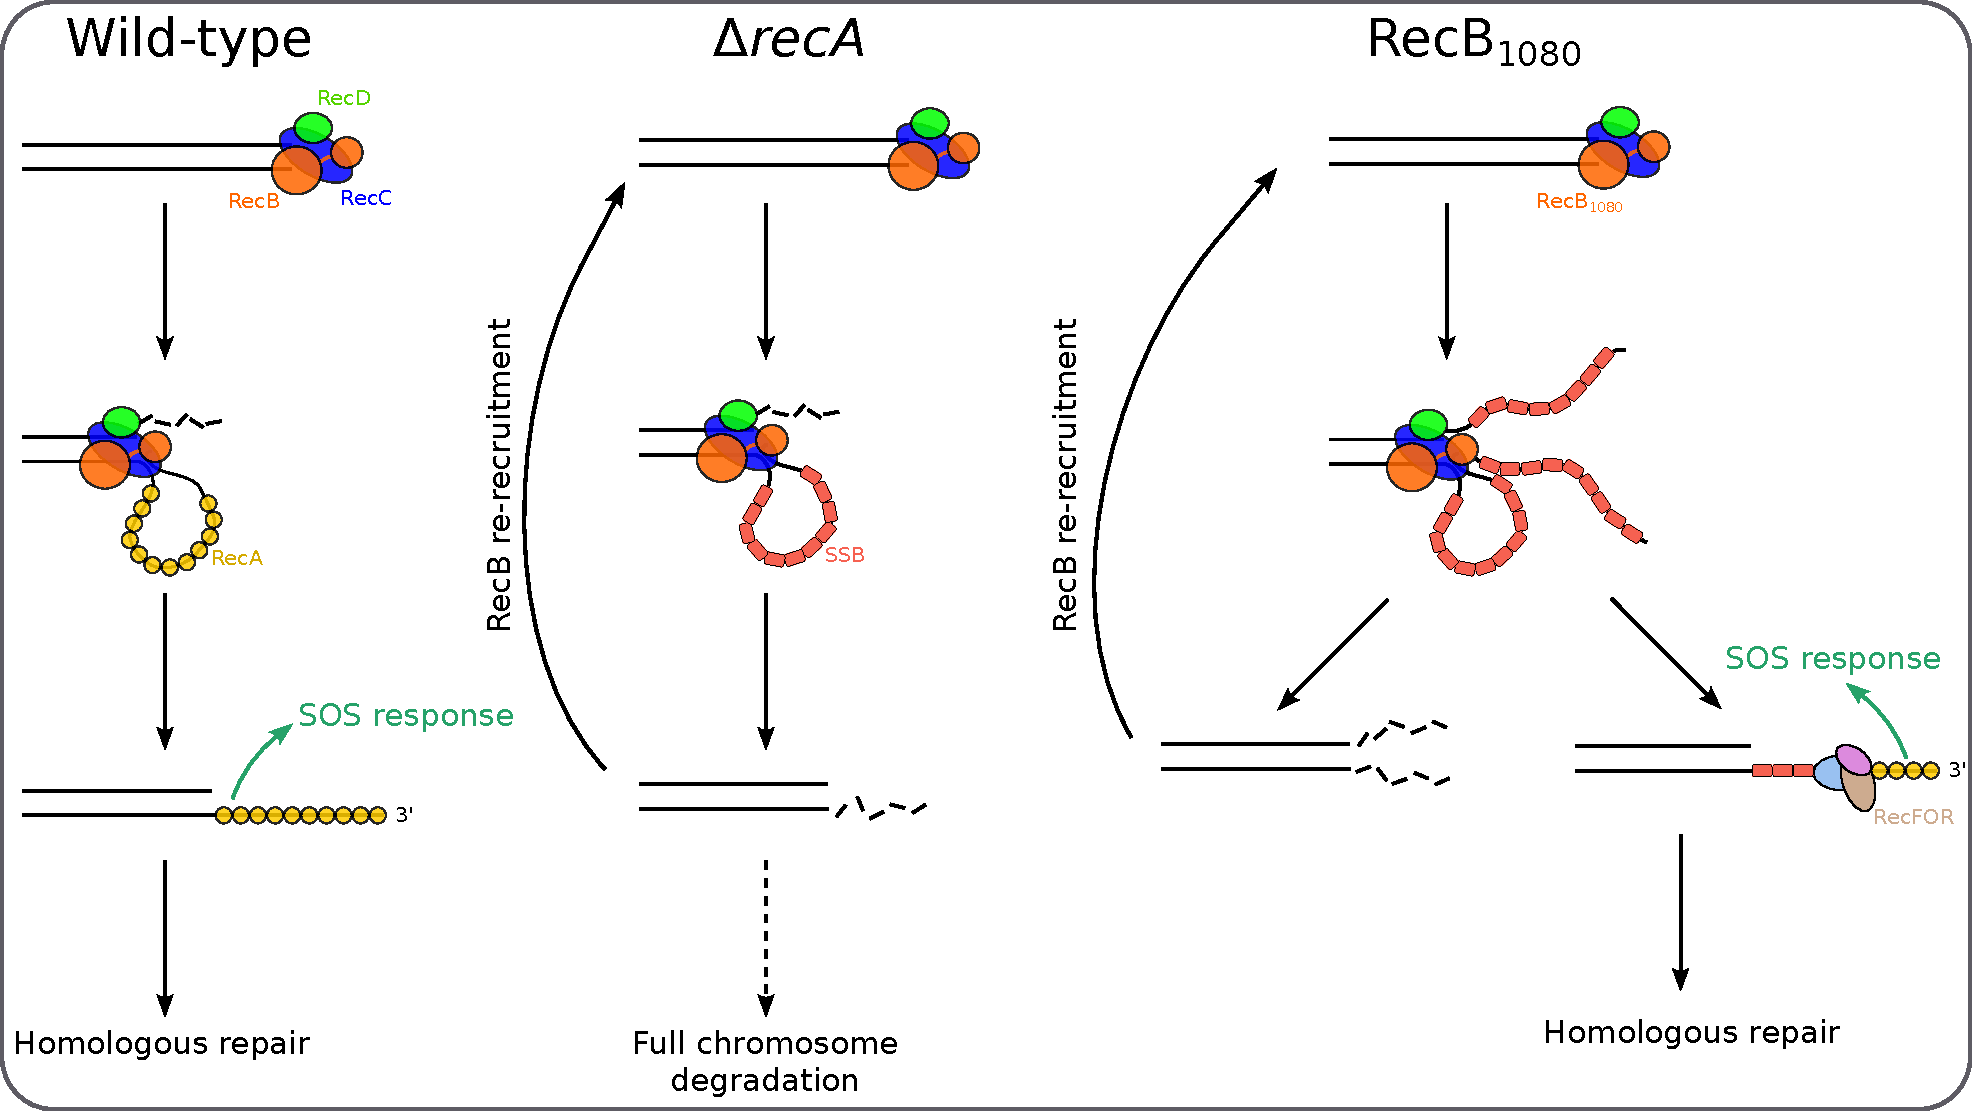
\includegraphics[width=\textwidth]{Figures/Fig_mutants_pathways.pdf}
    \caption{RecBCD recruitment pathways in wild-type \emph{E. coli}, \dreca\ and \teneighty\ mutants. \textbf{(Wild-type)} After DSB recognition, RecBCD degrades DNA until it recognises a Chi-site. It switches activity to create a 3' ssDNA overhang, and promotes RecA loading. The RecA-coated ssDNA can then be used for DNA repair by homologous recombination. \textbf{($\mathbf{\Delta}$reca)} In the absence of RecA, the 3' ssDNA is coated by SSB, and eventually digested by cellular nucleases. Blunting of the DNA end by digestion of the ssDNA creates a new substrate for binding of RecBCD. \textbf{(RecB$\mathbf{_{1080}}$)} Following DSB recognition, \teneighty\ unwinds DNA without digesting it. The unwound ssDNA can either be digested by nucleases, leading to a new blunt dsDNA end and RecBCD re-recruitment; or the RecFOR complex displaces SSB to load RecA, allowing DNA repair by homologous recombination to proceed.}
    \label{Fig:pathways}
\end{figure*}

Our observations of cell elongation (Figure \ref{Fig:mutants}A), RecB recruitment to DNA (Figure \ref{Fig:mutants}C), and nucleoid position (Figure \ref{Fig:mutants}D) in the different mutant strains have led us to the model of RecB recruitment described in Figure \ref{Fig:pathways}. In wild-type cells, a DSB is recognised by RecBCD, which promotes RecA loading. The RecA filament triggers the SOS response, and is used for homology search and repair. In the \dreca\ mutant, the 3' ssDNA generated by RecBCD is first coated by SSB, and then degraded by cellular nucleases. This leads to blunting of the DNA end, creating a new substrate on which RecBCD can bind. This circle leads to multiple RecBCD recruitments per DSB, and eventually to full chromosome degradation. In the \teneighty\ mutant, RecBCD unwinds DNA without degrading it. After the ssDNA is coated with SSB, two competing pathways take place: either DNA degradation by nucleases leading to DNA-end blunting and re-recruitment of RecBCD, or displacement of SSB by RecFOR and loading of RecA, leading to SOS induction and homologous repair.